\chapter{$k$-Analytic Curves}

In this chapter, we aim to further develop intuition surrounding the structure of analytic spaces.
Whereas giving an explicit picture for higher dimensional $k$-analytic spaces is difficult, curves have the advantages that they yield visualisations as in the case of the affine line.
The theory of $k$-analytic curves is a rich field of study, and presently we will focus on studying curves and their \textit{skeleta} through formal models.

\section{Generic Fibers of Formal Schemes}

We first give an overview of the theory of formal schemes, following \parencite[Chapter~7]{boschformal}.
Recall that a topological ring $A$ is said to have an $\mathfrak{a}$-adic topology, where $\mathfrak{a}$ is an ideal of $A$, if the subsets $\mathfrak{a}^n$ form a basis of neighbourhoods of $0$.
The $\mathfrak{a}$-adic completion for such a ring is defined as $\hat{A} = \varprojlim_{n} A/\mathfrak{a}^n$; the resulting ring is Hausdorff and complete.
Where $\mathfrak{b}$ is an ideal such that $\mathfrak{a}^n \subset \mathfrak{b}$ and $\mathfrak{b}^n \subset \mathfrak{a}$ for some $n$, then the topologies generated by the two ideals are equivalent, and any such ideal $\mathfrak{b}$ is known as an ideal of definition of $A$.

Now assume $A$ is a complete and Hausdorff $\mathfrak{a}$-adic ring.
Similarly to the $\operatorname{Spec}$ construction, the affine building blocks are given by $\spf A$, the formal spectrum. As a topological space, $\operatorname{Spf} A$ is given by
the underlying topological space of $\spec A/\mathfrak{a}$ and hence, it consists of open prime ideals of $A$.
We endow $\spf{A}$ with a structure sheaf $\sheaf_{\spf{A}}$ where for each open $U \subset \spf{A}$, we define 
\[
    \sheaf_{\spf{A}}(U) = \varprojlim \sheaf_{\spec{A/\mathfrak{a}^n}}(U)
\]
where the inverse limit is taken in the category of topological rings, and the topology on each $\sheaf_{\spec{A/\mathfrak{a}^n}}(U)$ is discrete.
The right hand side of the expression is well defined, since for all $n > 0$, the immersion $\spec A/\mathfrak{a}^n \to \spec{A/\mathfrak{a}}$ is a homeomorphism.
Generally, a formal scheme is then a locally topologically ringed space where each point has an open neighbourhood isomorphic to an affine formal scheme.
Morphisms of formal schemes are morphisms in the category of locally topologically ringed spaces.

We are interested particularly in a certain class of formal schemes, of which we now give an overview following \parencite[\S 5.2.1]{temk}.
Fix a non-zero element $\pi$ of the maximal ideal of $R$, which is then a $\pi$-adic ring.
Let $R\{T_1, \dots, T_n\}$ be the algebra given by $k\{T_1, \dots, T_n\} \cap R[[T_1, \dots, T_n]]$.
Hence, it consists of formal power series over $R$ in $n$ variables which converge on the closed unit disc.
We say an $R$-algebra $A$ is of \textit{topologically finite presentation} (tfp) if it is isomorphic to the algebra $R\{T_1, \dots, T_m\}/I$, for some finitely generated ideal ideal $I$.
In addition, $A$ is called \textit{admissible} if it is tfp and it does not have $\pi$-torsion.
If $A$ is tfp, then it can be shown that $A \otimes_{R} k$ is a $k$-affinoid algebra admitting an admissible epimorphism $k\{T_1, \dots, T_n\} \to A \otimes_{R} k$, for some $n$.
We will say that a formal $R$-scheme $\fmodel$ is locally finitely presented (lfp), resp. admissible, if $\fmodel$ has a locally finite cover by open affine formal schemes of the form $\spf A$, where $A$ is tfp, resp. admissible.

Let $X$ be a $R$-scheme with a locally finite covering by open subschemes $\spec A$, where each $A$ is finitely presented as a $R$-algebra.
Then, we can define the formal completion $\hat{X}$ as follows. 
Let $\mathfrak{J}$ be the quasi-coherent ideal sheaf generated by $\pi$.
Then, $\hat{X}$ is defined as a topological space to be the topological space underlying the closed subscheme $Y$ of $X$ cut out by $\mathfrak{J}$, with the sheaf of topological rings $\sheaf_{\hat{X}} = \varprojlim \sheaf_{X}/\mathfrak{J}^{n}$, where each sheaf $\sheaf_{X}/\mathfrak{J}^{n}$ is restricted to $Y$ along the inclusion $Y \to X$.
Locally, let $X = \spec A$; then $\hat{X}$ is given by $\spf{\hat{A}}$, where $\hat{A}$ is the completion of $A$ with respect to the ideal $\pi A$.

For a lfp formal scheme $\fmodel$, we define its \textit{special fiber} $\fmodel_s := \fmodel \times_{R} \tilde{k}$, where the fiber product is taken in the category of formal schemes.
Then, $\fmodel_s$ is a scheme locally of finite presentation over $\tilde{k}$. 
Locally, the special fiber of $\fmodel = \spf{A}$ is given by the scheme $\spec{A/\maxideal A}$.

Furthermore, we assign to an lfp formal scheme $\fmodel$ a $k$-analytic space $\fmodel_{\eta}$, known as the generic fiber of $\fmodel$.
Firstly, if $\fmodel = \spf A$, then we set $\fmodel_{\eta} = \berkspec{A \otimes_{R} k}$.
A map $\spf A \to \spf B$ corresponds to a continuous homomorphism $B \to A$, which induces a homomorphism of $k$-affinoid algebras $B \otimes_{R} k \to A \otimes_{R} k$ and hence of $\berkspec{A \otimes_{R} k} \to \berkspec{B \otimes_{R} k}$.

Next, assume $\fmodel$ is separated and choose a locally finite covering by open affine formal subschemes $\{ \fmodel_{i} \}_{i \in I}$.
Then, each intersection $\fmodel_{ij} = \fmodel_i \cap \fmodel_j$ is also an affine open formal subscheme.
It is a fact that if $\mathfrak{Y} \to \fmodel$ is an open immersion of affine formal schemes, then $\mathfrak{Y}_{\eta} \to \fmodel_\eta$ is the embedding of an affinoid domain.
Hence, we may glue the affinoid spaces $\{ (\fmodel_{i})_{\eta} \}_{i \in I}$ along the affinoid domains $\{ (\fmodel_{ij})_{\eta} \}_{i, j \in I}$ using \cref{gluing}.
A morphism $\mathfrak{Y} \to \fmodel$ of separated formal schemes induces a morphism $\mathfrak{Y}_{\eta} \to \fmodel_\eta$ by gluing the induced morphisms $(\mathfrak{Y}_i)_{\eta} \to \fmodel$, where $\{\mathfrak{Y}_i\}$ is a locally finite covering by open affine formal subschemes.

If $\fmodel$ is arbitrary with a covering $\{ \fmodel_i \}_{i \in I}$ by separated formal schemes, then the intersections $\fmodel_{ij}$ are separated formal schemes, and it can be shown that $(\fmodel_{ij})_{\eta}$ is a compact analytic domain in $(\fmodel_i)_{\eta}$ and $(\fmodel_j)_{\eta}$.
We may therefore glue $(\fmodel_i)_{\eta}$ and $(\fmodel_j)_{\eta}$ along $(\fmodel_{ij})_{\eta}$ as before to obtain $\fmodel_{\eta}$.
Since affinoid and compact analytic domains are closed subsets in a Hausdorff space, the fact that the cover is locally finite is necessary to perform the gluing.
Similarly to the separated case, we may also define a morphism of $k$-analytic spaces $\mathfrak{Y}_{\eta} \to \mathfrak{X}_{\eta}$ for any morphism $\mathfrak{Y} \to \mathfrak{X}$ by gluing appropriately.
It may then be verified that $\eta$ gives a functor, known as the generic fiber functor.

There is a canonical reduction map $\operatorname{red}_{\fmodel}: \fmodel_\eta \to \fmodel_s$ which is defined by the following procedure. 
Let $x \in \fmodel_\eta$ be a point and $\spf{A} \subset \fmodel$ such that $(\spf{A})_\eta$ contains $x$.
Then $x$ defines a character $A \otimes_{R} k \to \resfield$ and hence a homomorphism $A \to A \otimes_{R} k \to \resfield$.
The following lemma shows that the image of this map lands inside $\resfield^{\circ}$.

\begin{lemma}\label{lemma:ringfactors} \parencite[Exercise 5.2.2.6]{temk}
    Suppose $A$ is a tfp $R$-algebra, generated by $f_1, \dots, f_n$.
    Then for all $x \in (\spf{A})_{\eta}$ and $1 \leq i \leq n$ we have $|f_i|_x \leq 1$.
\end{lemma}
\begin{proof}
    We may find an admissible epimorphism $\phi: k\{T_1, \dots, T_n\} \to A \otimes_{R} k$ such that $T_i \mapsto f_i$ for each $i$.
    Denote $\mathbb{B}^{n} = \berkspeck{t_1, \dots, t_n}$.
    Then the morphism $\phi$ induces a map $\phi^{*}: \berkspec{A \otimes_{R} k} \to \mathbb{B}^n$, where a point $x \in \berkspec{A \otimes_{R} k}$ gives a point $\phi^{*}(x) \in \mathbb{B}^n$ by the equation $|f|_{\phi^{*}(x)} = |\phi(f)|_x$.
    Hence, we see that $|f_i|_x = |\phi(t_i)|_x = |t_i|_{\phi^{*}(x)} \leq 1$, where the final inequality follows from the fact that the norm $||\cdot||$ on $k\{t_1, \dots, t_n\}$ is such that $||t_i|| = 1$, and any element of the Berkovich spectrum is bounded by this norm.
\end{proof}

\Cref{lemma:ringfactors} shows that $x \in (\spf A)_{\eta}$ induces a map $A \to \resfield^{\circ}$ where the image of the ideal $\pi A$ lands in $\resfield^{\circ \circ}$.
Hence, there is a well-defined map $A/\pi A \to \resresfield$.
Then, $\red{\fmodel}{x}$ is defined to be the point given by $\spec \resresfield \to \fmodel_s$.
This map is anti-continuous, in that the inverse image of an open (resp. closed) set is closed (resp. open).

If $X$ is an $R$-scheme locally of finite presentation, there are now two ways to obtain a $k$-analytic space: either by taking the generic fiber of the formal completion $\hat{X}_{\eta}$ or by taking the analytification of the generic fiber $\anl{X_k}$, where $X_k := X \times_{R} k$.
In general, there is a canonical map $\i_{X}: \hat{X}_{\eta} \to \anl{X_{k}}$, which we can construct as follows \parencite[\S 5.3]{bconrad}.
By the universal property of analytification, it suffices to give a map of locally ringed spaces $\hat{X}_{\eta} \to X_{k}$. Consider the case where $X = \spec A$ is affine, for some finitely generated $R$-algebra $A$.
There is a canonical map $A \otimes k \to \hat{A} \otimes k$ and it is a standard result that $\operatorname{Hom}(Y, X) \cong \operatorname{Hom}(\Gamma(X, \sheaf_X), \Gamma(Y, \sheaf_Y))$ for a locally ringed space $Y$ and an affine scheme $X$ \parencite[Tag 01I1]{stacks-project}. 
Hence, we immediately obtain a map $\hat{X}_{\eta} \to X_k$, which gives the desired morphism $i_X: \hat{X}_{\eta} \to \anl{X_k}$.
This morphism is `functorial' in the following sense: if $X \to Y$ is a morphism of affine schemes, then we have an induced commuting square \footnote{This may be more formally stated by saying that $i_X$ is a functor from the category of affine schemes to the arrow category of $k$-analytic spaces.}:
\[
\begin{tikzcd}
 & \hat{X}_{\eta} \arrow[r] \arrow[d] & \anl{X_k} \arrow[d] \\
 & \hat{Y}_{\eta} \arrow[r] & \anl{Y_k}
\end{tikzcd}
\]
This follows from the fact that for any morphism $A \to B$ of finitely presented $R$-algebras, the following square commutes.
\[
\begin{tikzcd}
 & A \otimes k \arrow[r] \arrow[d] & \hat{A} \otimes k \arrow[d] \\
 & B \otimes k \arrow[r] & \hat{B} \otimes k
\end{tikzcd}
\]



As in the case of constructing the generic fiber functor, we may extend this map first to the case where $\hat{X}$ is a separated formal scheme, and then to the case where $\hat{X}$ is non-separated, to obtain a functorial canonical morphism $i_X$ for any scheme $X$ locally of finite presentation over $R$.

\begin{example}
    Let $X = \mathbb{A}^{1}_{R}$. Then we find that $\anl{X_k} = \affline$, while $\hat{X}_{\eta} = \berkspec{k\{t\}}$ is the unit disk. 
    In this case, $i_X : \berkspec{k\{t\}} \xhookrightarrow{} \affline$ is the canonical embedding of the closed unit disk into the affine line.
\end{example}

\begin{example}
    Let $X$ be the affine line over $R$ with doubled origin. 
    As a scheme, this is formed by gluing the affines $\spec R[T]$ and $\spec R[S]$ by identifying the opens $\spec R[T, T^{-1}], \spec R[S, S^{-1}]$ using the isomorphism $T \mapsto S$. The space $X_k$ is then the analytic affine line with doubled origin. 
    However, the generic fiber of the formal completion of $X$ is a little more interesting: it is in fact the closed unit disk with doubled open unit disk which we previously encountered as an example of a generalized space which is not good space.
    The map $i_X$ then identifies $\hat{X}_{\eta}$ with the closed unit disk in the affine line with doubled origin.
    Except for the origin, each point lying on an open unit disk and its copy are both identified with the same point in $\anl{X}_k$.
    Hence, $i_X$ is not injective.
\end{example}

The following lemmas and theorems, adapted from \parencite[Exercise 5.2.3.1]{temk} describe the map $i_X$ more generally. 
The details of these facts are often omitted in the literature, so we provide some proofs.

\begin{lemma}\label{lemma:affinecaseisaffinoid}
    If $X$ is an affine scheme of finite presentation, then $i_X$ is the embedding of an affinoid domain.
\end{lemma}
\begin{proof}
    Let $X = \spec A$.
    Suppose $A$ is generated by $f_1, \dots, f_n$.
    Then, we may fix an admissible epimorphism $k\{T_1, \dots, T_n\} \to \hat{A} \otimes_{R} k$ mapping $T_i \mapsto f_i$.
    By \parencite[Corollary 2.3.2]{berk1}, the induced map \[\hat{X}_{\eta} = \berkspec{\hat{A} \otimes_{R} k} \to \mathbb{B}^{n} = \berkspeck{T_1, \dots, T_n}\] is a closed immersion, that is, it is the embedding of an analytic domain with closed image.

    The functoriality of $i_X$ then induces the following commuting diagram:
    \[
    \begin{tikzcd}
        \hat{X}_{\eta} \arrow[d] \arrow[r,"i_X"]  & \anl{X_k} \arrow[d] \\
        \mathbb{B}^n \arrow[r] & \mathbb{A}^{n, \operatorname{an}}_{k}
    \end{tikzcd}
    \]
    where the vertical and bottom maps are closed immersions of $k$-analytic spaces.
    Since the vertical and bottom maps are injective, it follows that $i_X$ is also injective.
    Since the source is compact and the target is Hausdorff, $i_X$ is a homeomorphism onto its image.
    Now let $Z \to \anl {X_k}$ be a morphism of $k$-analytic spaces such that the image is contained in $\hat{X}_{\eta} \subset \anl X$.
    It follows that there is an induced map $Z \to \affnspace$ with the image contained in $\mathbb{B}^{n} = \berkspec{k\{T_1, \dots, T_n\}}$, hence there is a induced map $Z \to \mathbb{B}^{n}$ since $\mathbb{B}^{n}$ is an affinoid domain in $\affnspace$.
    Furthermore, the map $Z \to \mathbb{B}^{n}$ has image contained in $\hat{X}_{\eta}$, so since $\hat{X}_{\eta}$ is an analytic domain in $\mathbb{B}^{n}$, we conclude that there is a map $Z \to \hat{X}_{\eta}$.
    Since each induced map was uniquely determined by the map $Z \to \anl X$, it follows that the map $Z \to \hat{X}_{\eta}$ is unique, so that $i_X: \hat{X}_{\eta} \to \anl X$ is the embedding of an affinoid domain.
\end{proof}

\begin{lemma}\label{lemma:genericfibercharacterization}
    The points $y \in \hat{X}_{\eta}$ are in bijection with the set of maps $\spec{\resfieldof{x}^\circ} \to X$ extending the map $\spec{\resfieldof{x}} \to X$, where $x = i_X(y)$.
\end{lemma}
\begin{proof}
    Fix a point $y \in \hat{X}_{\eta}$ and let $i_X(y) = x$. 
    Now let $\spec A$ be an affine open in $X$ such that $y \in (\spf{\hat{A}})_{\eta}$, from which it follows that $i_X(y) = x \in \anl{(\spec A_k)}$.
    By \cref{lemma:affinecaseisaffinoid}, the restriction of $i_X$ to $(\spf{\hat{A}})_{\eta}$ is the embedding of an affinoid domain into $\anl{(\spec{A_k})}$; since the completed residue field may be computed within an affinoid domain containing the point, it follows that $\resfieldof{y} \cong \resfield$. 
    
    Next, we consider the map 
    \[A \to \hat{A} \otimes_{R} k \to \resfieldof{y} \cong \resfieldof{x}.\]
    The image of $A$ along this map lands in $\resfieldof{y}^\circ \cong \resfield^\circ$ by lemma~\ref{lemma:ringfactors}, so that there is a factorisation $A \to \resfieldof{x}^{\circ}$.
    This gives a lift $\spec{\resfield^\circ} \to \spec{A} \xhookrightarrow{} X$.
    
    Conversely, suppose that such a lift exists. Then, the image of $\spec{\resfield^\circ} \to X$ is contained within some affine open $\spec A$, since $\resfield^\circ$ is local. 
    Hence, we have a homomorphism $A \to \resfield^\circ$, which, by passing to completions, determines a homomorphism $\hat{A} \to \resfield^{\circ}$ and subsequently a map $\hat{A} \otimes_{R} k \to \resfield$. 
    This is a character corresponding to some point $y \in (\spf{\hat{A} \otimes_{R} k})_\eta \xhookrightarrow{} \hat{X}_\eta$. Since the map $\spec{\resfield^\circ} \to X$ extends the map $\spec{\resfield} \to X$, it follows by construction of $i_X$ that $i_X(y) = x$.
    
    The two procedures are verified to be inverses of each other.
\end{proof}

\begin{theorem}\label{separatedix}
If $X$ is separated and quasi-compact then the map $i_X$ is the embedding of a compact analytic domain.
\end{theorem}
\begin{proof}
The valuative criterion of separatedness indicates that there exists at most one lift $\spec{\resfield^{\circ}} \to X$ of a map $\spec{\resfield} \to X$. 
Hence, by \cref{lemma:genericfibercharacterization}, $i_X$ is injective. 
The source is compact since it is a finite union of affinoid domains which are compact and the target is Hausdorff, hence, it must be a homeomorphism onto its image.
At each point $y \in \hat{X}_{\eta}$ there exists an affinoid neighbourhood $V$ of $y$ in $\hat{X}_{\eta}$ such that the restriction of $i_X$ to $V$ is the embedding of an affinoid domain $V \to \anl{X}$, hence $i_X(\hat{X}_{\eta}) \subset \anl X$ is such that each point has an affinoid neighbourhood in $i_X(\hat{X}_{\eta})$.
It follows that $i_X$ is the embedding of an analytic domain.
\end{proof}

\begin{corollary} \label{properisiso}
If $X$ is proper over $R$, then there is an isomorphism $i_X: \hat{X}_\eta \xrightarrow{\sim} \anl{X_k}$.
\end{corollary}
\begin{proof}
The valuative criterion of properness indicates that there exists precisely one lift $\spec{\resfield^{\circ}} \to X$ of a map $\spec{\resfield} \to X$. 
By \cref{lemma:genericfibercharacterization}, it follows that $i_X$ is surjective, and since $X$ is necessarily separated, we find that $\hat{X}_\eta$ is an analytic domain in $\anl{X}_k$, so that $i_X$ is an isomorphism.
\end{proof}

Letting $X = \mathbb{P}^{1}_{R}$, we find that $\hat{X}_{\eta}$ is the gluing of two closed disks $\berkspec{k\{T\}}$ and $\berkspec{k\{S\}}$ along the isomorphism $\berkspec{k\{T, T^{-1}\}} \cong \berkspec{k\{S, S^{-1}\}}$ given by $T \mapsto S^{-1}$.
On the other hand, $\anl X$ is the gluing of two copies of $\affline$ along the isomorphism $\anl{\mathbb{G}_{m, k}} \cong \anl{\mathbb{G}_{m, k}}$ given by $T \mapsto T^{-1}$.
\Cref{properisiso} finally shows that the two constructions are isomorphic.

In this example, the formal scheme $\hat{X}$ can be considered as a \textit{formal model} for the $k$-analytic space $\anl{X}$.

\begin{defn}
    A formal $R$-model $\fmodel$ for a $k$-analytic space $X$ is an admissible formal $R$-scheme equipped with an isomorphism $\fmodel_{\eta} \cong X$.
\end{defn}

As we will see, models are spaces capturing the geometry of the $k$-analytic space in a (formal) scheme which is potentially easier to study.
If $X$ is a proper $k$-scheme locally of finite type, then $\anl{X}$ admits a formal model \parencite[Remark 5.3.3.2]{temk}.

\section{Skeleta of $k$-Analytic Curves}

\subsection{Classification of Points}

To begin, we must consider the notion of dimension, which is more subtle for $k$-analytic spaces than in the case of schemes.
An obstruction is the fact that for $k$-affinoid algebras, the Krull dimension is not preserved under extension of the base field.
An example of this, as found in \parencite[\S 3.5]{temk}, is the $k$-affinoid algebra $K_r := k\{r^{-1} T, rT^{-1}\}$.
For $r \not\in \sqrt{|k^{\times}|}$, $K_r$ is a field, and hence has Krull dimension $0$, but $K_r \hat{\otimes}_{k} K_r \cong K_r\{T\}$ does not.
This motivates the following definition.

\begin{defn} \parencite[\S 2.3]{berk1}.
    The dimension $\dim(X)$ of a $k$-affinoid space $X = \berkspec{\banr}$ is the Krull dimension of the algebra $\banr \hat{\otimes}_{k} K$, where $K$ is a non-Archimedean field extension of $k$ such that there exists an admissible epimorphism $K\{T_1, \dots, T_n\} \to \banr \hat{\otimes}_{k} K$.
\end{defn}

 It can be shown that such a field extension exists, and that $\dim(X)$ is independent of the choice of extension.
 We extend this notion to a general $k$-analytic space $X$, by defining its dimension $\dim(X)$ to be the supremum of the dimensions of the $k$-affinoid domains of $X$.
 
 Following \parencite{bpr}, we define a $k$-analytic curve to be the analytification of a smooth, proper, geometrically connected algebraic curve over $k$.
 We caution the reader that other sources map give more a general definition, which may require more theory to be built up, but our definition will capture all the cases we are interested in.
 It can be shown that such a space is of dimension one by invoking the appropriate GAGA theorems \parencite[Corollary 3.2.8]{berk1} \parencite[Proposition 3.4.3]{berk1}.

The classification of points for the affine line may then be extended to more general curves.
For each valued extension $k \subset K$, we associate the parameters:
\begin{align*}
    & E(K) = \dim_{\QQ}\left(|K^{\times}|/|k^{\times}| \otimes_{\ZZ} \QQ\right) \\
    & F(K) = \operatorname{tr.deg.}(\tilde{K} / \tilde{k}).
\end{align*}

Let $X$ be a $k$-analytic space of dimension $n$.
Fixing a point $x \in X$, we denote $E(x) := E(\resfield)$ and $F(x) := F(\resfield)$.
Then, it may be shown that $E(x) + F(x) \leq n$ \parencite[Lemma 2.5.2]{berk93}.
In the case where $n = 1$, we can then classify $x$ as follows \parencite[\S 2.3.3]{temk}:
\begin{enumerate}
    \item $x$ is type I if $\resfield \subset \widehat{k^a}$, where $\widehat{k^a}$ is the completed algebraic closure of $k$;
    \item $x$ is type II if $E(x) = 0$ and $F(x) = 1$; 
    \item $x$ is type III if $E(x) = 1$ and $F(x) = 0$;
    \item $x$ is type IV if $E(x) = F(x) = 0$ and $x$ is not of type I.
\end{enumerate}

Note that if $x$ is type I then $E(x) = F(x) = 0$.
It may be verified that this is an extension of our earlier classification of the points of the affine line over an algebraically closed field.

\subsection{Skeleta of Annuli}

For the rest of this chapter, we assume that $k$ is algebraically closed.

Recall that we defined maps $\evt: \affline \to \mathbb{R}_{\geq 0}$ and $\sigma: \mathbb{R}_{\geq 0} \to \affline$, where $\evt(x) = |T|_x$ and $\sigma(r) = \zeta_{0, r}$.
Using these maps, we were able to define several analytic domains in $\affline$, including \textit{standard open} and \textit{standard closed} annuli, denoted by $\annulus{a, b}_{+}$ and $\annulus{a, b}$ respectively, for some $a, b \in k^{\times}$ with $|a| \leq |b|$.
When $b = 1$, we will denote the annulus as $\annulus{a}$.
Denoting $c = ab^{-1}$, we have a series of isomorphisms:
\[\annulus{a, b} \cong \annulus{c} \cong \berkspec{k\{t, |c| \cdot t^{-1}\}} \cong \berkspec{k\{t, s\}/(st - c)}. \]
If $X$ is any $k$-analytic space which is isomorphic to a standard closed (resp. open) annulus, then we will call $X$ a \textit{generalized closed} (resp. \textit{generalized open}) annulus.
A standard annulus is any standard open or standard closed annulus, and a generalized annulus is any space which is either a generalized open or a generalized closed annulus.
Similarly, if $X$ is isomorphic to a standard closed (resp. open) ball, then $X$ will be called a \textit{generalized closed} (resp. \textit{generalized open}) ball.


Next, recall that we defined a strong deformation retraction from $\affline \to \sigma(\mathbb{R}_{\geq 0})$.
In order to obtain a suitable notion of a skeleton for an arbitrary curve, we make a similar definition for an annulus.

\begin{defn}\parencite[\S 2.3]{bpr}
    For any standard closed or open annulus $A$, its \textit{skeleton} is the subset \[\Sigma(A) := \sigma(\evt(A)). \]
\end{defn}

There is then a map $\rho_A := \sigma \circ \evt$ which is a retraction of $A$ onto $\Sigma(A)$, and can be shown to be a strong deformation retraction \parencite[Proposition 4.1.6]{berk1}.
If $X$ is a generalized annulus, then fixing an isomorphism $\phi: X \to A$ for some standard annulus $A$, then the skeleton $\Sigma(X)$ of $X$ is defined as $\phi^{-1}(\Sigma(A))$, and there is a corresponding retraction $\rho_X = \phi^{-1} \circ \rho_A \circ \phi$.
It can be shown that $\Sigma(X)$ and $\rho_X$ do not depend on $A$ or $\phi$ \parencite[Corollary 2.6]{bpr}.

The following lemma describes the retraction map.

\begin{lemma} \label{annulusretract} \parencite[Lemma 2.12]{bpr}
    Let $A$ be a generalized annulus. 
    Then $A \backslash \Sigma(A)$ is an analytic domain in $A$ isomorphic to an infinite disjoint union of open balls.
    If $\overline{B}$ is the topological closure of an open ball $B$ in the disjoint union, then $\overline{B} \backslash B = \{ x \}$, and for every point $y \in B$, we have $\rho_{A}(y) = x$.
\end{lemma}

Before giving the proof, we consider the standard closed annulus \[\annulus{1} = \berkspeck{t, t^{-1}} \cong \berkspec{k\{s, t\}/(s t - 1)}.\]
Then, the affine formal scheme $\fmodel = R\{s, t\}/(st - 1)$ is such that $\fmodel_{\eta} \cong \annulus{1}$, and hence $\fmodel$ is a formal $R$-model for $\annulus{1}$.
In this case, $\fmodel_s \cong \spec \tilde{k}[s, t]/(st - 1)$ is the affine open subscheme of the affine line over $\tilde{k}$ given by removing the origin, and we wish to describe $\operatorname{red}_{\fmodel}$ explicitly.
Firstly, consider the point $x = \zeta_{0, 1} \in \berkspeck{t, t^{-1}}$.
Then $\resresfield \cong \tilde{k}(t)$, and the map $\tilde{k}[t, t^{-1}] \to \tilde{k}(t)$ is the natural map.
The kernel of this map corresponds to the zero ideal, hence $\red{\fmodel}{x}$ is the generic point of $\fmodel_s$.
Next, assume that $x \in D(b, 1)$ for some $b \in R^{\times}$.
The claim is that $\red{\fmodel}{x}$ is the point given by the maximal ideal $(t - \tilde{b})$, where $\tilde{b}$ is the residue class of $b$ in $\tilde{k}$.
Indeed, we see that $|t - b|_x < 1$, so that $(t - \tilde{b}) \subset \ker (\tilde{k}[t, t^{-1}] \to \resresfield)$.
By maximality of $(t - \tilde{b})$ and the fact that the kernel of the map $\tilde{k}[t, t^{-1}] \to \resresfield$ is a prime ideal as $\resresfield$ is a field, it follows that the inclusion is an equality.

\begin{proof}[Proof of \cref{annulusretract}]
    We elaborate on the proof given in \textit{loc. cit.}
    If $A = \annulus{1}$, then the first two claims follow by the remarks preceding the proof and the fact that $\tilde{k}$ is infinite.
    The last statement is a consequence of the anti-continuity of $\operatorname{red}_{\fmodel}$.
    Indeed, let $B$ be an open ball as in the statement, so $\red{\fmodel}{b} = \{y \}$ for all $b \in B$, where $y$ is a closed point.
    If $z \in \overline{B}$, then $z$ is contained in any closed set containing $B$.
    Now let $U$ be any open in $\fmodel_s$ containing $y$; then $\operatorname{red}^{-1}_{\fmodel}(U)$ is a closed set and so it contains $z$.
    Therefore, $U$ contains $\red{\fmodel}{z}$.
    Since $U$ was arbitrary, it follows that $z \in \operatorname{red}^{-1}_{\fmodel}(\xi)$, where $\xi$ is the generic point of $\fmodel_s$.
    Hence, $z = \zeta_{0, 1}$.
    
    Next, assume $A$ is any generalized annulus, and by fixing an isomorphism, we may assume it is a standard annulus.
    Let $r \in \evt(A)$.
    If $r \not\in |k^{\times}|$, then we claim that $\evt^{-1}(r)$ is a single type III point $x$.
    Indeed, if $y$ is any point such that $|T|_y = r$, then for any $b \in k$ we have $|T - b|_y = \max \{ |T|_y, |b| \} = |T - b|_x$, so that $y = x$.
    Hence it suffices to consider when $r \in |k^{\times}|$. 
    In this case, we may rescale so that $r = 1$, in which case $\evt^{-1}(r) = \annulus{1}$.
    It then suffices to show that the connected components of $\annulus{1} \backslash \{ \zeta_{0, 1} \}$ are the connected components of $A \backslash \Sigma(A)$ since then we reduce to the previous case.
    This follows if $\annulus{1} \backslash \{ \zeta_{0, 1} \}$ is both open and closed in $A \backslash \Sigma(A)$.
    It is closed since $\annulus{1}$ is closed, and $\annulus{1} \backslash \{ \zeta_{0, 1} \} = \annulus{1} \cap (A \backslash \Sigma(A))$, and it is open since it is a union of open balls of the form $D(b, 1)$.
\end{proof}

\subsection{Semistable Vertex Sets and Semistable Reduction}

Assuming $X$ is a smooth proper connected algebraic curve over $k$, we now develop the theory of semistable vertex sets following \parencite[\S 3-4]{bpr}, which allow the notion of a skeleton of an annulus to be used to construct a skeleton for $\anl X$.

Note that in the case of an annulus $\mathbb{S}(a, b)$, the skeleton is determined completely by the type II points $\zeta_{0, |a|}$ and $\zeta_{0, |b|}$ which form the endpoints, since the skeleton is then the unique path between the two points.
Removing these two points results in a disjoint union of an open annulus $\mathbb{S}(a, b)_{+}$ and infinitely many open balls.
This observation motivates the following definitions.

\begin{defn} \parencite[Definition 3.1]{bpr}
    A semistable vertex set $V$ of $X$ is a finite set of type II points $V \subset \anl X$ such that $\anl X \backslash V$ is a disjoint union of open balls and finitely many generalized open annuli.
    Such a decomposition is called a \textit{semistable decomposition}.
\end{defn}

\begin{defn} \parencite[Definition 3.3]{bpr}
    If $V$ is a semistable vertex set for $X$, then the skeleton of $X$ with respect to $V$ is
    \[
        \Sigma(X, V) = V \cup \bigcup \Sigma(A)
    \]
    where $A$ runs over the generalized open annuli in the semistable decomposition induced by $V$.
\end{defn}

Next, we would like to define a retraction map $\anl X \to \Sigma(X, V)$ for any semistable vertex set $V$, with the aid of the following result.
Although the result is a generalisation of \cref{annulusretract}, its proof requires some additional theory on meromorphic functions on analytic spaces and hence is omitted.

\begin{lemma} \parencite[Lemma 3.4]{bpr}
    Let $V$ be a semistable vertex set for $X$ and $B$ a connected component of $\anl{X} \backslash \Sigma(X, V)$.
    Then $B$ is isomorphic to an open ball, and if $\overline{B}$ is the topological closure of $B$ in $\anl X$, then $\overline{B}\backslash B = \{ x \}$ for some point $x \in \Sigma(X, V)$ known as the limit boundary of $B$.
\end{lemma}

As a corollary, we see that $\Sigma(X, V)$ is a closed subset of $\anl X$.

We now define a retraction map $\rho_{V}: \anl X \to \Sigma(X, V)$ with respect to $V$  by setting $\rho_{V}(x) = x$ for any $x \in \Sigma(X, V)$ and $\rho_{V}(x)$ to be the limit boundary of the connected component of $\anl{X} \backslash \Sigma(X, V)$ containing $x$.

\begin{lemma}\parencite[Lemma 3.8]{bpr}
The retraction $\rho_{V}$ is a continuous map which agrees with the retraction $A \to \Sigma(A)$ when restricted to an open annulus in the semistable decomposition induced by $V$.
\end{lemma}
\begin{proof}
    By \cref{annulusretract}, $\rho_V$ is continuous on any open annulus $A$ in the semistable decomposition, and agrees with $\rho_{A}$ by \cref{annulusretract}.
    We now show continuity, completing the part of the proof which was left as an exercise in \textit{loc. cit.}.
    Fixing $x \in V$, let $U \subset \Sigma(X, V)$ be an open neighbourhood of $x$ in $\Sigma(X, V)$.
    It suffices to show that $x$ lies in the interior of $\rho_V^{-1}(U)$.
    By shrinking $U$, we may assume that each connected component $U_i$ of $U \backslash \{ x \}$ is contained in an open annulus $A_i$ in the semistable decomposition.
    Then $A'_i  = \rho_V^{-1}(U_i)$ is an open annulus.
    Let $\{B_j\}$ be the open balls in the semistable decomposition which retract to $x$.
    The claim is that 
    \[
        \{ x \} \cup \bigcup B_j \cup \bigcup A'_i
    \]
    is an open neighbourhood of $x$. 
    Consider its complement $Y$ in $\anl X$; then $Y \cap (\anl X  \backslash \bigcup A_i)$ is closed, and the set $Y \cap A_i$ is closed in $A_i$ by the continuity of the restriction map on each open annulus.
    It follows that $Y$ is closed.
\end{proof}

The language of semistable vertex sets can be seen as a translation of the theory of semistable models of a curve into the analytic setting.

\begin{defn}\parencite[\S 4]{bpr}
    A \textit{semistable formal $R$-curve} is an integral admissible formal $R$-curve $\fmodel$ such that the special fiber $\fmodel_s$ is a connected reduced algebraic curve over $\tilde{k}$ where all singularities are ordinary double points.
    A \textit{semistable formal model for $X$} is a semistable formal $R$-curve with an isomorphism $\fmodel_\eta \cong \anl{X}$.
\end{defn}

A recurring motif is that the geometry of an analytic space can be determined by the structure of the special fiber of a suitable model.
As a first encounter, we look at a powerful theorem of Bosch-L{\"u}tkebohmert, extended by Berkovich to the setting of $k$-analytic spaces, which generalizes our earlier observations regarding the map $\operatorname{red}_{\fmodel}: \annulus{1} \to \spec \tilde{k}[T, T^{-1}]$.

\begin{theorem} \label{boshlutkebohmert} \parencite[Prop. 2.3]{boschlutkebohmert} \parencite[Theorem 4.3.1]{berk1} Let $\fmodel$ be an integral formal $R$-model for an analytic curve $\anl X$ with a reduced special fiber $\fmodel_s$. 
Fix a point $x \in \fmodel_s$ and denote by $F_x := \operatorname{red}^{-1}_{\fmodel}(x)$ the \textit{formal fiber} over $x$. Then:
    \begin{enumerate}
        \item $x$ is the generic point of an irreducible component if and only if $F_x$ consists of a single type II point.
        \item $x$ is a smooth closed point if and only if $F_x$ is isomorphic to a standard open ball.
        \item $x$ is an ordinary double point if and only if $F_x$ is isomorphic to a standard open annulus.
    \end{enumerate}
\end{theorem}

It follows from this theorem and the anticontinuity of the reduction map that to any semistable formal model $\fmodel$, the set $V(\fmodel)$ of type II points $\operatorname{red}_{\fmodel}^{-1}(\xi)$ as $\xi$ runs over the generic points of $\fmodel_s$ is a semistable vertex set.
The reverse also holds: any semistable vertex set gives rise to a semistable formal model.

\begin{theorem}\label{semistablecorrespondence} \parencite[Theorem 4.11]{bpr}
    The correspondence $\fmodel \mapsto V(\fmodel)$ is a bijection between the set of semistable formal models of $X$ up to isomorphism and the set of semistable vertex sets of $X$.
\end{theorem}

We omit the proof, which may be found in \textit{loc. cit.} and instead walk through some examples of how the inverse map is constructed.
The general proof is not much more difficult than our explicit examples, and we will sketch how the proof generalises in each case.
There is a key difference between the case of the projective line and other curves \parencite[Remark 4.17]{bpr}.
Firstly, recall that for a field extension $k \subset K$ there exists a curve $C(K)$ over $k$ unique up to isomorphism with function field $K$.
Define the genus of a type II point $x$ to be the genus of $C(\resresfield)$.
Any type II point in $\projlinean$ has genus $0$.
If $x$ is a type II point in $\anl{X}$ of positive genus, then it must be contained within any semistable vertex set of $\anl{X}$, since otherwise it has a neighbourhood isomorphic to an open ball or open annulus which admit embeddings into $\projlinean$.

The proof is split into several cases, and we exemplify each case here by considering $X = \mathbb{P}^{1}_{k}$, fixing a semistable vertex set $V$ and denoting by $\Sigma$ its associated skeleton.

\paragraph{$\Sigma$ consists of a single vertex.}

To exemplify this, let $V = \{ \zeta_{0, 1} \}$.
In this case, $\projlinean \backslash V$ is an infinite disjoint union of open balls.
Let $B_1 = D(0, 1)$ and $B_2 = D(\infty, 1)$.
The complements $Y_1 = X \backslash B_1$ and $Y_2 = X \backslash B_2$ are then the affinoid domains given by the closed balls $E(\infty, 1) \cong \berkspeck{S}$ and $E(0, 1) \cong \berkspeck{T}$ respectively.
We have models for $Y_1$ and $Y_2$ given by $\spf R\{T\}$ and $\spf R\{S\}$ respectively.
The intersection $Y_1 \cap Y_2$ is the affinoid domain $\berkspeck{T, T^{-1}} \cong \berkspeck{S, S^{-1}}$, where the isomorphism is induced by $T \mapsto S^{-1}$.
The intersections inform us how to glue the formal models for $Y_1$ and $Y_2$: we have open subsets $\spf R\{T, T^{-1}\} \subset \spf R\{T\}$ and $\spf R\{S, S^{-1}\} \subset \spf R\{S\}$.
Gluing along the isomorphism $\spf R\{T, T^{-1}\} \cong \spf R\{S, S^{-1}\}$ given by $T \mapsto S^{-1}$ recovers the semistable formal model $\hat{\mathbb{P}}^{1}_{R}$ given by the formal completion of $\mathbb{P}^{1}_{R}$ that we have previously encountered.

More generally, we fix two distinct balls $B_1, B_2$ in the semistable decomposition and let $Y_1 = \anl{X} \backslash B_1$ and $Y_2 = \anl{X} \backslash B_2$.
Then $Y_1$ and $Y_2$ are affinoid domains due to the following lemma, the proof of which we omit due to its dependence on some aspects of the theory of which we have not given a comprehensive treatment.

\begin{lemma} \label{complementaffinoid} \parencite[Lemma 4.12]{bpr}
    Let $X$ be a projective $k$-curve and $Y \subset \anl X$ an open analytic domain isomorphic to either an open ball or an open annulus.
    Then $\anl{X} \backslash Y$ is an affinoid domain in $\anl{X}$.
\end{lemma}

Then, we find models for $Y_1, Y_2$ and $Y_1 \cap Y_2$ by the following lemma.

\begin{lemma} \label{canonicalmodel} \parencite[Proposition 1.1]{boschlutkebohmert}
    Let $\berkspec{\banr}$ be a reduced $k$-affinoid space and assume $k$ is algebraically closed.
    Then the ring
    \[\banr^{\circ} = \{ f \in \banr \; \vert \; |f|_x \leq 1 \; \text{for all} \; x \in \berkspec{\banr} \}\]
    is a tfp $R$-algebra and for $\fmodel = \spf \banr^{\circ}$, we have $\fmodel_{\eta} \cong \berkspec{\banr}$.
\end{lemma}

In our current setting, $k$ is algebraically closed and $X$ is smooth, hence reduced.
It follows by \parencite[Proposition 3.4.3]{berk1} that $\anl{X}$ is also reduced, in the sense that all local rings are reduced. 
In particular any affinoid domain $\berkspec{\banr}$ in $\anl{X}$ is reduced.
Furthermore, $\banr$ has no $\pi$-torsion since it is a $k$-algebra, and it follows from this that $\banr^{\circ}$ is an admissible $R$-algebra.
Hence, $\fmodel$ is an admissible formal model for $\berkspec{\banr}$, called the \textit{canonical model}.

Gluing the canonical models for $Y_1$ and $Y_2$ along the canonical model for $Y_1 \cap Y_2$ then gives us the desired semistable formal model.

\paragraph{$\Sigma$ consists of a single edge.}
For this case, we can take $V = \{x = \zeta_{0, r}, y = \zeta_{0 , 1} \}$, where $0 < r < 1$ and $r = |c|$ for some $c \in |k^{\times}|$.
Let $B_x = D(0, r)$ and $B'_x = D(c, r)$, and similarly $B_y = D(\infty, 1)$ and $B'_y = D(1, 1)$.
We see that $Y$ is the standard annulus $\mathbb{S}(c)$ which has a model $\mathcal{Y} = \spf{R\{S, T\}/(S T - c)}$.

We may perform a change of coordinates by setting
\[
    U := \frac{T - c}{T - 1}.
\]
where $T$ is the coordinate on $\mathbb{P}^{1}_{k}$. 
This induces an automorphism of $\mathbb{P}^{1}_{k}$, hence of $\projlinean$.
Assume that $x \in Y'$, so that $|T - 1|_x \geq 1$ and $|T - c|_x \geq r$.
Analysing each of the cases $r < |T|_x < 1, |T|_x \leq r, |T|_x \geq 1$, we find that $r \leq |U|_x \leq 1$.
From this it follows that the image of $Y'$ lands inside $\mathbb{S}(c)$.
Furthermore, the transformation is self-inverse, so performing a similar calculation shows that $\mathbb{S}(c)$ lands inside $Y'$ under the inverse map, hence showing that this transformation gives an isomorphism $Y' \cong \mathbb{S}(c)$.
Therefore, $\mathfrak{Y}' = \spf{R\{A, B\}/(A B - c)}$ is a model for $Y'$.

The intersection $Y \cap Y'$ is modelled by open formal subschemes $\mathfrak{U} \subset \mathfrak{Y}$ and $\mathfrak{U}' \subset \mathfrak{Y}'$.
By \cref{boshlutkebohmert}, the open subset $\mathfrak{U}$ is obtained from $\mathfrak{Y}$ by removing the closed points $\red{\mathfrak{Y}}{B'_x}$ and $\red{\mathfrak{Y}}{B'_y}$.
These correspond to the ideals of $\tilde{k}[S, T]/(S T)$ given by $(T - 1, S)$ and $(T, S - 1)$ respectively.
Similarly, the open subset $\mathfrak{U}'$ is obtained from $\mathfrak{Y}'$ by removing the closed points $\red{\mathfrak{Y}'}{B_x}$ and $\red{\mathfrak{Y}'}{B_y}$ corresponding to the ideals
of $\tilde{k}[A, B]/(A B)$ given by $(A - 1, B)$ and $(A, B - 1)$ respectively.
The isomorphism $\mathfrak{U} \to \mathfrak{U}'$ is then induced by the homomorphism of rings sending $A \mapsto T/(T - 1)$ and $B \mapsto S/(S - 1)$.
It follows that the resulting formal model consists of two copies of $\mathbb{P}^{1}_{\tilde{k}}$ intersecting transversally.

The general procedure is similar: we begin by choosing two open balls $B_x, B_x'$ retracting to $x$ and two open balls $B_y, B_y'$ retracting to $y$.
Again, by \cref{complementaffinoid}, $Y = \projlinean \backslash (B_x \cup B_y)$ and $Y' = \projlinean \backslash (B'_x \cup B'_y)$ are affinoid domains, and we let $\mathfrak{Y}$ and $\mathfrak{Y}'$ be the respective canonical models.
It can be shown that each model consists of two curves intersecting at an ordinary double point.
The intersection $Y \cap Y'$ is an affinoid domain, and the canonical model is identified with an open formal subscheme of each model by deleting a smooth point from each irreducible component of the model.
Gluing along these opens then gives the desired formal model.

\paragraph{$\Sigma$ consists of at least two edges.}

Let $V = \{\zeta_{0, 1}, \zeta_{0, r}, \zeta_{0, r'} \}$, where $0 < r' < r < 1$ and $r = |c|, r' = |c'|$ for some $c, c' \in k$.
The induced semistable decomposition contains open annuli $\mathbb{S}(c', c)_+$ and $\mathbb{S}(c, 1)_{+}$.
Then, $\Sigma$ has edges $e_1$ and $e_2$ corresponding to the annuli $A_1 = \mathbb{S}(c', c)$ and $A_2 = \mathbb{S}(c, 1)$ respectively.
Denote the vertices by $x = \zeta_{0, 1}$, $y = \zeta_{0, r}$ and $\zeta_{0, r'} = z$.

Firstly, we consider the edge $e_1$ with vertices $x$ and $y$.
The open ball $B_x = D(0, r')$ retracts to $x$, and $\projlinean \backslash (A_2 \cup B_x)$ is the standard annulus $A_1$, which has a model $\mathfrak{Y} = \spf {R\{S, T\}/(S T - d)}$ where $d = c' c^{-1}$.
We note that $\rho_V^{-1}(x) = E(0, r')$, which has model $\mathfrak{Y}_x = \spf {R\{U\}}$.
We find that $B_x$ is the formal fiber above the closed point $\zeta$ given by the origin of the special fiber of $\mathfrak{Y}_x$.
Suppose that $\mathfrak{C}_x = \spec \tilde{k}[T]$ is the irreducible component of $\mathfrak{Y}$ such that the generic point of $\mathfrak{C}_x$ has formal fiber $\{x\}$.
Let $\xi$ be the closed point where the irreducible components of $\mathfrak{Y}_1$ intersect.
The intersection $A_1 \cap E(0, r')$ is modelled by the open formal subscheme $\mathfrak{C}_x \backslash \{ \xi \}$ of $\mathfrak{C}_x$ and $\mathfrak{Y}_x \backslash \{ \zeta \}$ of $\mathfrak{Y}_x$.
We then have an isomorphism
\[
    \mathfrak{C}_x \backslash \{ \xi \} \cong \mathfrak{Y}_x \backslash \{ \zeta \}
\]
which is induced by the mapping $U \mapsto T^{-1}$.
Gluing along this isomorphism results in a formal scheme $\fmodel_1$ topologically given by a projective line over $\tilde{k}$ intersecting transversally with an affine line.

We may perform a similar procedure for the edge $e_2$ and the vertex $z$, resulting in an isomorphic formal scheme $\fmodel_2$.
It now remains to glue the two formal schemes.
To do this, we let $\mathfrak{D}_1$ be the irreducible component of $\fmodel_1$ whose generic point has formal fiber $\{y\}$, and similarly define $\mathfrak{D}_2$ with respect to $\fmodel_2$.
Topologically, $\mathfrak{D}_1$ is homeomorphic to $\spec \tilde{k}[S]$, and $\mathfrak{D}_2$ is homeomorphic to $\spec \tilde{k}[V]$.
Let $\xi_1$ and $\xi_2$ be the ordinary double points of the special fibers of $\fmodel_1$ and $\fmodel_2$ respectively.
Then, we see that the formal fibers above $\mathfrak{D}_1 \backslash \{ \xi_1 \}$ and $\mathfrak{D}_2 \backslash \{ \xi_2 \}$ are both given by the affinoid domain given by $A_1 \cap A_2 \cong \annulus{1}$.
We therefore glue $\fmodel_1$ and $\fmodel_2$ along the following isomorphism
\[
\mathfrak{D}_1 \backslash \{ \xi_1 \} \cong \spf{R\{S, S^{-1}\}} \cong \spf{R\{V, V^{-1}\}} \cong \mathfrak{D}_2 \backslash \{ \xi_2 \}
\] 
where the middle isomorphism maps $S \mapsto V^{-1}$.
This procedure results in a projective line with a projective line intersecting transversally at $0$ and another projective line intersecting transversally at infinity, visualised in \cref{fig:semistable}.

\begin{figure}
    \centering
    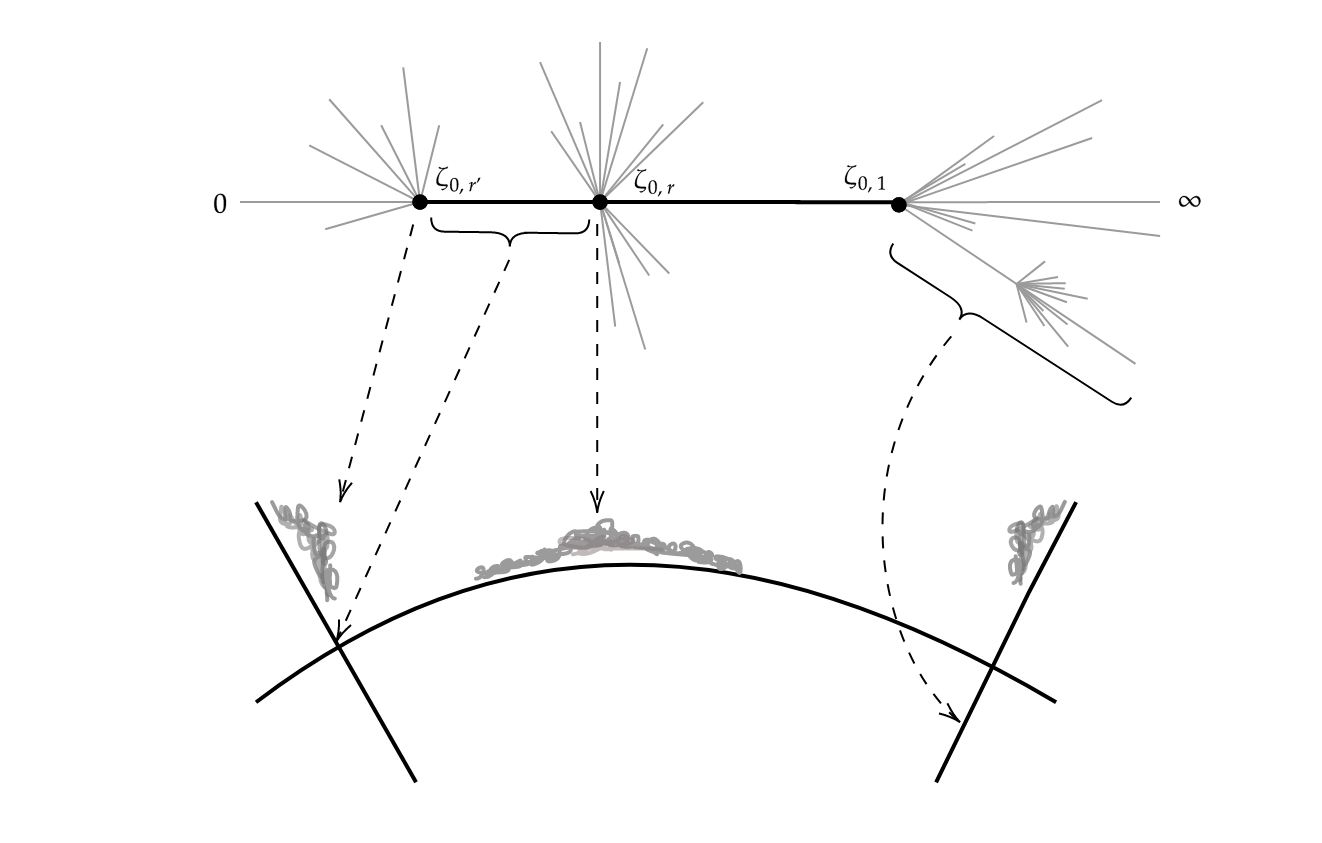
\includegraphics[width=0.8\textwidth]{Images/semistable.png}
    \caption{The relationship between a skeleton induced by a semistable vertex set and the corresponding formal model. The top image shows the analytic projective line with the skeleton in bold. Dashed arrows indicate the reduction map. 
    Clouds above each projective line in the semistable model shown at the bottom indicate the generic point of the component.}
    \label{fig:semistable}
\end{figure}

In the general case, we begin by fixing an edge $e$.
Suppose the open annuli in the semistable decomposition are $A_0, \dots, A_n$, and by permuting indices that $e$ contains $\rho(A_0)$.
There are two cases to consider. 

If $e$ has a vertex $x$ which is not contained in any other edge in $\Sigma$ \footnote{Note that this case is missing from the proof of  \parencite[Theorem 3.2.10]{bpr}.}, then we choose an open ball $B_x$ retracting to $x$.
It can be shown that $Y = \rho^{-1}(x)$ is an affinoid domain, by arguing that $\anl{X} \backslash (\bigcup_{i = 0}^{n} A_i)$ is an affinoid domain using \cref{complementaffinoid} and using the fact that $\rho^{-1}(x)$ is a connected component.
We let $\mathfrak{C}_x$ be the canonical model for $\rho^{-1}(x)$.
Similarly, we can show that $Y' = \rho^{-1}(e) \backslash B_x$ is an affinoid domain with canonical model $\mathfrak{Y}$, by arguing that it is a connected component of $\anl{X} \backslash (B_x \cup \bigcup_{i = 1}^{n} A_i)$.
The intersection $Y \cap Y'$ is then modelled by isomorphic open formal subschemes of $\mathfrak{C}_x$ and $\mathfrak{Y}$, giving the appropriate gluing data.

In the second case, both vertices of $e$ are contained in other edges of $\Sigma$.
We again argue that $\rho^{-1}(e)$ is an affinoid domain since it is a connected component of $\backslash (\bigcup_{i = 1}^{n} A_i)$.
Let $\mathfrak{D}$ be the canonical model; then the formal fibers above closed points are given by connected components of $\rho^{-1}(e) \backslash \{x, y \}$.
These connected components are the open balls which retract to either $x$ or $y$, or $A_0$, so it follows that $\mathfrak{D}$ consists of two irreducible components intersecting at an ordinary double point $\xi$.
If $\mathfrak{C}$ is the irreducible component whose generic fiber has formal fiber $\{x\}$, then the canonical model for $\rho^{-1}(x)$ is given by $\mathfrak{C} \backslash \{\xi\}$.
If $e'$ is another edge with vertex $x$, then $\rho^{-1}(e) \cap \rho^{-1}(e') = \rho^{-1}(x)$, so that by repeating this procedure for $e'$, we obtain the necessary gluing data for the respective canonical models.

A natural question to ask now is whether any $k$-analytic curve has a semistable decomposition, and hence, a skeleton. 
The following theorem answers this positively in the algebraically closed case.

\begin{theorem}[Semistable Reduction Theorem] \parencite[Theorem 7.1]{boschlutkebohmert}
    Let $X$ be a smooth, projective, geometrically connected curve over $k$, where $k$ is not necessarily algebraically closed.
    Then, there exists a finite extension $k \subset k'$ with valuation ring $R'$ such that $\anl{(X \times_{k} k')}$ admits a semistable formal $R'$-model.
\end{theorem}

Hence, when $k$ is algebraically closed, we deduce by our correspondence that a $k$-analytic curve $\anl{X}$ has a semistable vertex set.
